\documentclass{article}
\usepackage{code,a4wide}

\usepackage{graphics,epsfig,epic,eepic,epsfig}

\setlength{\parskip}{0.25cm}
\setlength{\parsep}{0.25cm}
\setlength{\topsep}{0cm}
\setlength{\parindent}{0cm}
\renewcommand{\textfraction}{0.2}
\renewcommand{\floatpagefraction}{0.7}


% Terminology
\newcommand{\block}{block}
\newcommand{\Block}{Block}
\newcommand{\segment}{segment}
\newcommand{\Segment}{Segment}
\newcommand{\step}{step}
\newcommand{\Step}{Step}

\newcommand{\note}[1]{{\em $\spadesuit$ #1}}

\begin{document}
\title{Implementation of Retainer Profiling}
\author{Sungwoo Park and Simon Peyton-Jones}

\makeatactive
\maketitle

\section{Retainer Profiling}

Retainer profiling~\cite{CN} is a profiling technique which is based upon a 
special view of production and consumption of heap objects at runtime:
while producers build heap objects to form new pieces of graph,
consumers hold pointers to these heap objects, or \emph{retain} them, so 
that they are not freed during garbage collections. 
On this basis, we refereed to such consumers as \emph{retainers}.
Notice that an object can have more than one retainer because it can
be pointed to by multiple objects.

For each live object in the heap, retainer profiling computes 
all its retainers, or its \emph{retainer set}.
A naive implementation of retainer profiling could consider every
immediate ancestor of an object as its retainer.
Although this approach appears to provide an accurate report on the 
relationship between retainers and retainees, the result can hardly be useful.
For instance, it is pointless to scrutinize a list and treat each cons
cell as a retainer of the following cons cell.
This observation suggests that we need to have a way of designating only 
certain types of objects as candidates for retainers.
In other words, we need to employ an oracle which tells whether a given
object can be a retainer or not.

Since no retainer of a particular object needs to be using the
object actively, we can find all its retainers simply by traversing
the graph. In other words, we do not have to distinguish those retainers
actively exploiting it from other retainers just holding pointers
to it (either directly or indirectly).
Thus, retainer profiling can be accomplished simply by traversing the
graph.

Figure~\ref{fig-retaineralgorithm} shows the algorithm for retainer
profiling. The traversal begins at every root, and proceeds 
in a depth first manner (or a breadth first manner).
The function @R()@ returns the \emph{identity} of a given retainer such
as its information table address or
the name of the module which creates it.
Notice that the retainer identity function does not need to be a 
one-to-one mapping:
multiple objects can share the same identity.
Such a retainer identity function reduces the cost of traversal.
For instance, when an object
is reached from several retainers which share the same identity, we need to
consider only the first visit to the object.
In other words, whichever retainer (among those sharing the same identity) 
leads to the object for the first time affects the retainer set of the object
in consideration
and all the other retainers can be ignored.
Thus, the more coarse the function @R()@ is, the less
it costs to traverse the graph for retainer profiling.
The function @isRetainer()@ tells whether a given object is a retainer or not.
Hence, the behavior of the retainer profiling algorithm is parameterized
over: 1) the set of roots; 2) the function @R()@; 3) the function
@isRetainer()@.

One important invariant on the function @R()@ is that its return value
must be consistent for a given retainer. In other words, @R()@ must return
the same value for a given retainer no matter it is invoked.
For this reason, the memory address of a retainer, for instance, cannot be used as
its retainer identity because its location may change during garbage collections.

\begin{figure}[ht]
\begin{center}
\begin{code}
for every root r
  retain(r, r)

R(r) =
  the identity of r

isRetainer(c) =
  if c is a retainer then   
    true 
  else 
    false

retain(c, r) =
  if R(r) is a member of c.retainerSet then 
    return
  add R(r) to c.retainerSet
  if isRetainer(c) then 
    r' := c
  else 
    r' := r
  for every successor c' of c
    retain(c', r')
\end{code}
\caption{Retainer profiling algorithm}
\label{fig-retaineralgorithm}
\end{center}
\end{figure}

Another way of formulating retainer profiling is in terms of fixed point
equations on retainer sets.
To be specific, given the two functions @isRetainer()@ and @R()@,
the retainer set of every object is computed as the least fixed point
solution of the following equations:
\begin{itemize}
\item For every root @r@, 
\begin{center}
  @R(r)@ $\in$ @r.retainerSet@.
\end{center}
\item For every reachable object @c@, 
\begin{center}
$\bigcup_{\mathit{each\ ancestor\ @a@\ of\ @c@}}$ @from(a)@ $\subseteq$ 
@c.retainerSet@ 
\end{center}
where @from(a)@ returns retainer(s) obtainable from @a@:
\begin{center}
@from(a)@ = if @isRetainer(a)@ then $\{@a@\}$ else @a.retainerSet@.
\end{center}
\end{itemize}

This document describes the implementation of retainer profiling on
the Glasgow Haskell Compiler runtime system. 
It explains every detail of the development so that it can be (hopefully)
a complete maintenance guide.
A secondary goal is to help (hopefully) those who wish to extend the system 
to implement another profiling scheme.\footnote{Unless otherwise mentioned,
all identifiers are defined in @RetainerProfile.c@ or @RetainerSet.c@.}

\section{Installing the GHC}

Installing the GHC is done as follows:

\begin{enumerate}
\item Get the source code from the CVS repository.
\begin{code}
./              cvs checkout fpconfig
./fptools/      cvs update -d CONTRIB common-rts distrib docs ghc glafp-utils 
                    hslibs literate mhms mk nofib testsuite
\end{code}

\item Set up the basic configuration.
\begin{code}
./fptools/      autoconf                    
./fptools/ghc/  autoconf
./fptools/      configure
\end{code}

\item Set up the configuration for development and debugging.
\begin{code}
./fptools/mk    vi build.mk
    GhcHcOpts = -O -fasm -Rghc-timing
    SplitObjs = NO
    GhcRtsHcOpts = 
    GhcRtsCcOpts = -g
    STRIP_CMD =:
\end{code}
@GhcLibWays@ tells the compiler to build the code for profiling as well.
@GhcRtsHcOpts@ has additional flags for @gcc@ when compiling @.hc@ files.
@GhcRtsCcOpts@ has additional flags for @gcc@ when compiling @.c@ files.
Since we will implement retainer profiling in @.c@ files, we turn on the 
debugging flag @-g@. 
The empty setting for @STRIP_CMD@ tells the compiler not to remove source code
information (generated due to the @-g@ option) from executable files so that
they can be examined with @gdb@.

\item Remove unnecessary files if needed and build everything.
\begin{code}
./fptools/      make
\end{code}
\end{enumerate}

\section{Adding Retainer Set Fields}

Since every Haskell closure now needs to store its retainer set at runtime, 
it must be augmented with a new field,
namely, a \emph{retainer set field}.
This section explains how to add such a field to Haskell closures.
It should be clear how to generalize the idea for adding 
any number of new fields.\footnote{The GHC provides two 
ways of building executable programs from 
source files: normal way and profiling way. 
We are concerned only about profiling way, and all the pieces of code 
implementing profiling way are wrapped by the @PROFILING@ 
pre-processing directive (as in @\#ifdef PROFILING@).
Therefore, all the additions and changes that we make to the source code 
are assumed to be wrapped by the @PROFILING@ pre-processing 
directive as well unless otherwise mentioned.}

\subsection{Adding a new field to Haskell closures} 

We want to add a retainer set field of type @retainerSet@ to every 
closure, so we create a new file @includes/StgRetainerProf.h@ where
we define the type @retainerSet@.
The actual definition of @retainerSet@ will be given later.

\begin{code}
/* includes/StgRetainerProf.h */
typedef ... retainerSet;
\end{code}

We make type @retainerSet@ to be publicly available by including
@includes/StgRetainerProf.h@ itself to @includes/Stg.h@ (not wrapped
by @PROFILING@).

\begin{code}
/* includes/Stg.h */
#include "StgRetainerProf.h"
\end{code}

Then we add a retainer set field @rs@ to the @StgProfHeader@ structure.

\begin{code}
/* include/Closures.h */
typedef struct {
   CostCentreStack *ccs;
   retainerSet *rs;
} StgProfHeader;
\end{code}

Now every closure @c@ (including static closures) has a retainer set field,
which can be accessed with @c->header.prof.rs@ (where @c@ denotes the 
address of the closure).

\subsection{Changing constants}

We are ready to reflect the new size of Haskell closures to other part
of the source code.
This is accomplished by changing a few constants which specify the size
of certain types of closures and their layout.

When building the runtime system, the @gcc@ compiler correctly figures out
the size of every structure on its own.
However, 
GHC simply reads @includes/Constants.h@ to to determine the size of 
closures assumed by the runtime system.
Thus, we must change the constants used by the GHC itself (as opposed to
the runtime system). They are all found in @includes/Constants.h@.
We increase each of them by 1 to reflect the retainer set field which is one 
word long:
\begin{code}
/* includes/Constants.h */
#define PROF_HDR_SIZE       2
#define SCC_UF_SIZE         5
#define SCC_SEQ_FRAME_SIZE  4
\end{code}
@PROF_HDR_SIZE@ denotes the size of the structure @StgProfHeader@, which
is now two words long. 
@SCC_UF_SIZE@ and @SCC_SEQ_FRAME_SIZE@ denote the size of the structures
@StgUpdateFrame@ and @StgSeqFrame@ (in @includes/Closures.h@) in
words.

Now we must rebuild the GHC so that, when executed, the code generated by 
the GHC must now allocate one more word for the retainer set field than before.

\begin{code}
./fptools/ghc/  make boot
./fptools/ghc/  make
\end{code}

The second command @make boot@ instructs the build system to analyze
the source code dependency so that the next execution of @make@ correctly
finds all required files.

Next we change four bitmap constants which specify the layout of
certain types of closures.
As an example, let us consider @RET_BITMAP@, which specifies the layout
of thunk selectors (corresponding to closure type @THUNK_SELECTOR@).
Without a retainer set field, there is only one non-pointer (represented
by $1$) followed by one or more pointers (represented by $0$) in the closure 
body and the bitmap representation is $0b1$, or $1$. 
With a retainer set field, which is not a pointer to another closure and thus
represented by $1$, there are two non-pointers, and the bitmap representation
is $0b11$, or $3$. Notice that the bitmap is interpreted in reverse order:
the least significant bit corresponds to the first word in the closure body,
and the second least significant bit to the second word, and so forth.
The same rule applies to the other three bitmap constants:
@CATCH_FRAME_BITMAP@ (for closure type @CATCH_FRAME@ and structure 
@StgCatchFrame@),
@STOP_THREAD_BITMAP@ (for closure type @STOP_FRAME@ and structure 
@StgStopFrame@), and
@UPD_FRAME_BITMAP@ (for closure type @UPDATE_FRAME@ and structure
@StgUpdateFrame@).

\begin{code}
/* rts/StgStdThunks.hc */
#define RET_BITMAP          3
/* rts/Exception.hc */
#define CATCH_FRAME_BITMAP  15
/* rts/StgStartup.hc */
#define STOP_THREAD_BITMAP  3
/* rts/updates.hc */
#define UPD_FRAME_BITMAP    7
\end{code}

For most closure types, the new definition of @StgProfHeader@ is
automatically propagated to their corresponding structures.
However, there are six closures types which are not affected by 
@StgProfHeader@. They are all stack closures:
@RET_DYN@, @RET_BCO@, @RET_SMALL@, @RET_VEC_SMALL@, @RET_BIG@, and
@RET_VEC_BIG@. 
If you want a new field to be added to these closures, you may
have to modify their corresponding structures.

\textbf{To do:} Presently the above changes introduce two bug in the 
runtime system. 
First, @nofib/real/symalg@ ends up with a division-by-zero
exception if we add a new field. 
Second, the runtime system option @-auto-all@ clashes in some test files
in the @nofib@ testing suite (e.g., @spectral/expert@).

\subsection{Initialization code}

When a new closure is allocated, its retainer set field may have to be 
initialized according to the way that retainer profiling is implemented.
For instance, we could use as an initial value a pointer to an empty retainer 
set. 
Alternatively we could assign a null pointer to indicate that its retainer
set has not been computed yet, which we adopt in our implementation.
In either case, we have to visit the new closure and execute some initialization
code on it so that its retainer set field is set to an appropriate value.

There are three parts in the source code which need to be modified.
dynamic closure initialization, static closure initialization,  
and update frame initialization.
The first is accomplished by modifying the macro @SET_PROF_HDR()@ (in 
@include/ClosureMacros.h@). When a closure  @c@ is created at runtime, 
@SET_PROF_HDR()@ is invoked immediately with @c@ as its first argument.
Thus, the following code initializes the retainer set field of every
dynamic closure to a null pointer.

\begin{code}
/* include/ClosureMacros.h */
#define SET_PROF_HDR(c,ccs_)            \
        ((c)->header.prof.ccs = ccs_, (c)->header.prof.rs = NULL)
\end{code}

Similarly, the macro @SET_STATIC_PROF_HDR()@ (in the
same file) specifies how the retainer set field of every static closure
is initialized, which is rewritten as follows:

\begin{code}
/* include/ClosureMacros.h */
#define SET_STATIC_PROF_HDR(ccs_)       \
        prof : { ccs : ccs_, rs : NULL },
\end{code}

\textbf{Obsolete:} Dynamic closures created through explicit C function invocations
(in @RtsAPI.c@) are now initialized by @SET_HDR()@.

%There is another way of creating dynamic closures through explicit C 
%function invocations at runtime. 
%Such functions are all defined in @RtsAPI.c@: @rts_mkChar()@, @rts_mkInt()@,
%@rts_mkWord()@, and so forth.
%Each function allocates memory for a new closure, 
%initializes it, and returns its address. 
%Therefore, we can simply insert in each function another initialization code 
%for retainer set fields.
%To this end, we define a macro @setRetainerField()@ and insert it 
%in each function:
%
%\begin{code}
%#define setRetainerField(p)             \
%  (p)->header.prof.rs = NULL
%\end{code}
%
%For instance, @rts_mkChar()@ is now defined as follows:
%
%\begin{code}
%/* RtsAPI.c */
%HaskellObj
%rts_mkChar (HsChar c)
%{
%  StgClosure *p = (StgClosure *)allocate(CONSTR_sizeW(0,1));
%  ...
%  setRetainerField(p);
%  return p;
%}
%\end{code}

Finally we may need to initialize the retainer set field of an update frame 
(stack closure) when it is pushed onto the stack for the first time. 
For instance, if we want to initialize the retainer set field of update
frames to a null pointer, we can rewrite the macro @PUSH_STD_CCCS()@ 
(in @includes/Updates.h@) as follows:

\begin{code}
/* includes/Updates.h */
#define PUSH_STD_CCCS(frame)            \
  (frame->header.prof.ccs = CCCS, frame->header.prof.rs = NULL)
\end{code}

In our implementation of retainer profiling, however, the retainer set field is not 
used for any stack closure.
Hence, the above modification is entirely unnecessary.
Also, update frames are the only exception to the standard way of creating
stack closures: all the other types of stack closures with a retainer set 
field are eventually initialized by
the macro @SET\_HDR()@ (in @includes/ClosureMacros.h@), which in turn
invokes @SET\_PROF\_HDR()@. This is not the case for update frames.
Compare @PUSH\_UPD\_FRAME()@ (in @includes/Updates.h@) and  
@PUSH\_SEQ\_FRAME()@ (in @includes/StgMacros.h@) for clarification.

\section{Retainer Sets}

At the end of retainer profiling, every live closure (except stack
closures, for which we do not compute retainer sets) is associated with
a retainer set; there can be no closure without an associated retainer set
because every live closure is visited during traversal.
Since many closures may well be associated with a common retainer set,
we want to avoid creating any particular retainer set more than once.
This section presents the details of manipulating retainer sets in our
implementation.

\subsection{Identity of a retainer}

The function @R()@ in Figure~\ref{fig-retaineralgorithm} returns
the identity of a retainer. In order to implement it, we need 
a type for retainer identity.
The type @retainer@ (in @includes/StgRetainerProf.h@) is introduced for
this purpose. 

There are various ways of defining the type @retainer@. 
For instance, we can designate the information table address of a retainer as
its identity as follows:

\begin{code}
struct _StgInfoTable;
typedef struct _StgInfoTable *retainer;
\end{code}

We can also use the cost centre stack associated with the retainer:

\begin{code}
typedef CostCentreStack *retainer;
\end{code}

The function @R()@ is embodied as the function @getRetainerFrom()@ in the 
implementation, whose type is @(StgClosure *)@ $\rightarrow$ @retainer@.
It is straightforward to define @getRetainerFrom()@ according to the definition
of @retainer@, as illustrated below:

\begin{code}
retainer getRetainerFrom(StgClosure *c) { return get_itbl(c); }
retainer getRetainerFrom(StgClosure *c) { return c->header.prof.ccs; }
\end{code}

\subsection{Retainer sets and the cost function}

A retainer set is stored in the structure @retainerSet@ 
(in @includes/StgRetainerProf.h@):

\begin{code}
typedef struct _retainerSet {
  nat num;
  nat cost;
  ...
  int id;
  retainer element[0];
} retainerSet;
\end{code}

The field @num@ gives the number of retainers in the retainer set, which
are all stored in the array @element[]@. Thus, the size of @element[]@
is assumed to be @num@.
The field @cost@ gives the sum of the \emph{costs} of those closures 
associated with the retainer set: if a closure @c@ is
associated with the retainer set, that is, if @c@ is retained by each
retainer in the retainer set and none else,
the cost of @c@ is added to the field @cost@. 
The field @id@ gives a unique identification number for the retainer set.

The interface to @retainerSet@ is as follows 
(see @RetainerSet.h@):

\begin{description}
\item[@void initializeAllRetainerSet(void)@] initializes the store for retainer sets.
\item[@void refreshAllRetainerSet(void)@] refreshes each retainer set by setting
its @cost@ field to zero. This function does destroy any retainer set.
\item[@void closeAllRetainerSet(void)@] destroys all retainer sets and closes
the store for retainer sets.
\item[@retainerSet *singleton(retainer r)@] returns a singleton retainer set
consisting of @r@ alone. If such a retainer set already exists, no new retainer
set is created. Otherwise, a new retainer set is created.
\item[@retainerSet *addElement(retainer r, retainerSet *rs)@] returns a retainer set
@rs@ augmented with @r@. If such a retainer set already exists, no new retainer set
is created. Otherwise, a new retainer set is created.
\item[@rtsBool isMember(retainer r, retainerSet *rs)@] returns a boolean value
indicating whether @r@ is a member of @rs@.
\item[@void traverseAllRetainerSet(void (*f)(retainerSet *))@] invokes the function
@f@ on every retainer set created.
\item[@void printRetainerSetShort(FILE *, retainerSet *)@] prints a single retainer
set.
\item[@void outputRetainerSet(FILE *, nat *allCost, nat *numSet)@] prints all 
retainer sets. Stores the sum of all their costs in @*allCost@ and the number
of them in @*numSet@.
\item[@void outputAllRetainerSet(FILE *)@] prints all retainer sets.
\end{description}

We also define a \emph{cost function}, which returns the cost of a given closure, 
in order to compute the field @cost@. 
The cost function can be defined in several ways.
A typical definition is on the size of a closure, which results in
the field @cost@ accumulating the size of all the closures retained by a
retainer set.
If we just want to count the number of closures retained by the
retainer set, we can simply set the cost of every closure to one regardless
of its closure type.
Furthermore, we can define the cost function flexibly according to
the closure type. 
For instance, we can set the size of any static closure to zero so that
it is not taken into account at all in computing the field @cost@. 
Notice that static closures are also visited during traversal because they 
may lead to other dynamic closures (e.g., static indirection closures of 
closure type @IND_STATIC@).
This is especially desirable because we usually focus on the heap use.
We can also selectively choose certain dynamic closure types not to contribute 
to the field @cost@.

In our implementation, there are two functions related with the cost function:
@cost()@ and @costPure()@. 
@cost()@ returns the size of the entire memory allocated for a given closure
(even including the two fields in the structure @StgProfHeader@). 
It returns zero for static closures. 
@costPure()@ returns the size of the memory which would be allocated for
a given closure with no profiling.
It is defined in terms of @cost()@, and it suffices to change only @cost()@
when a new scheme for the cost function is desired.
@costPure()@ is put to actual use in computing the field @cost@ because it 
effectively hides the memory overhead incurred by profiling.

\subsection{Implementation}

The algorithm for retainer profiling in Figure~\ref{fig-retaineralgorithm} 
adds at most one retainer to an existing retainer set (or an empty retainer set)
at any moment; it does not require a retainer set union operation.
This observation simplifies the implementation, and
we employ the following two functions for creating new retainer sets: 
@singleton()@, which creates a singleton retainer set, and 
@addElement()@, which adds an element to an existing retainer set. 

It is a frequent operation during retainer profiling to search for a retainer
set, which may or may not exist, built from a given retainer set and a
particular retainer.
To efficiently implement this operation,
we choose to store all retainer sets in a hash table and 
the structure @retainerSet@ is now extended with two new fields
@hashKey@ and @link@.
The field @hashKey@ stores the hash key which is obtained
from the retainers in a retainer set.
The field @link@ points to the next retainer set in the same bucket:

\begin{code}
typedef struct _retainerSet {
  ...
  StgWord hashKey;
  struct _retainerSet *link;
  ...
} retainerSet;
\end{code}

The hashing function must be defined in such a way that a retainer set
can have only one unique hash key regardless of the order its elements
are stored, i.e., the hashing function must be additive.

It is often observed that two successive executions of retainer profiling share
a number of retainer sets in common, especially if the two executions are
close in time.
This also implies that the number of all retainer sets which can be created
at any moment does not grow indefinitely regardless of the interval at which
retainer profiling is performed; it does not grow commensurately with the
number of times retainer profiling is executed.
This observation eliminates the need to free the memory allocated for
retainer sets; we can simply set the @cost@ field of every retainer set
to zero after each retainer profiling and reuse it during the next time.

\section{Graph Traversal}

At the heart of retainer profiling lies \emph{graph traversal};
the algorithm in Figure~\ref{fig-retaineralgorithm} is supposed to visit
every closure in the graph at least once and yield statistics on the heap use.
Since only live closures are reachable from the root, the algorithm
does not deal with dead closures.

This section presents details on how to achieve an efficient implementation of 
graph traversal without incurring extra memory overhead and compromising speed.

\subsection{Goal}

Traversing a graph itself can be done in a straightforward way;
we choose either depth first search or breadth first search, and traverse
the graph starting from a given set of roots.
After a complete traversal, each live closure @c@ (including static closures)
has an associated retainer set, whose address is stored in the field
@c->header.prof.rs@. 

A real complication arises when retainer profiling is performed once again:
all live closures which have survived all garbage collections since 
the previous retainer profiling 
still have an associated retainer set (indicated by
a non-null pointer in their retainer set field), which is no longer
valid. Any new closure created since then has
a null pointer in its retainer set field at the beginning of retainer 
profiling and will become associated with a retainer set.
Thus, we can no longer distinguish valid retainer set fields
from invalid ones. 

A simple remedy is to linearly scan the heap at the beginning of each 
retainer profiling and set all retainer set fields to a null pointer.
It resets the retainer set field of each dynamic closure, whether it is
live or not with respect to the given set of root.
This is feasible because any closure in the heap directly adjoins the
next closure, if any.
The problem is that we have no way of visiting all live static closures,
for which we compute retainer sets.

A moment of thought, however, reveals that we can completely avoid computing 
retainer sets for static closures. This is because retainer profiling is 
concerned only about the heap, which consists of dynamic closures and no
static closures. In other words, we can treat every static closure as
a bridge connecting two dynamic closures. 
For instance, if a dynamic closure @c@$_1$ has a pointer to a static
closure @s@ and @c@ has a pointer to another dynamic closure @c@$_2$,
we can think of the pointer in @c@$_1$ as a direct pointer to @c@$_2$.
The big problem is that if the graph has a cycle containing static closures,
an infinite loop occurs. In other words, we have no way of telling whether
a static closure has been visited or not and are forced to compute
retainer sets for static closures as well.\footnote{For instance, 
a static closure is allowed to have a self-reference in its SRT, which
is also followed during retainer profiling.}

Another remedy is to stores in every closure a time stamp for the
retainer set field. The time stamp indicates whether the retainer
set field is valid or no longer valid (i.e., it is for the previous
retainer profiling). 
At the cost of one extra field in each closure, we can achieve an
elegant implementation with little complication.
However, it turns out that the memory overhead is too big.\footnote{A typical
dynamic closure is only two or three words long.}
Thus, our goal is to stick to the definition of the structure @StgProfHeader@
given earlier and yet to achieve an elegant solution.

\subsection{Basic plan}

Since we visit every live object and update its retainer set field,
any retainer set field can either be valid (the corresponding retainer
set is valid) or point to a retainer set created during the previous
retainer profiling. 
In order to distinguish valid retainer set fields
from invalid ones, we exploit the least significant bit of the retainer
set field: we maintain a one bit mark which flips over every time
retainer profiling is performed, and judge that a retainer set field is
valid only if its least significant bit matches the mark.
The variable @flip@ serves for this purpose. 
The macros @isRetainerSetFieldValid()@ tests if the retainer set field
of a give closure @c@ is valid:

\begin{code}
#define isRetainerSetFieldValid(c) \
  ((((StgWord)(c)->header.prof.rs & 1) ^ flip) == 0)
\end{code}

As an example, a retainer set field can be set to a null value conforming
the current value of @flip@ by the macro @setRetainerSetToNull()@:

\begin{code}
#define setRetainerSetToNull(c)   \
  (c)->header.prof.rs = (retainerSet *)((StgWord)NULL | flip)
\end{code}

Now, when a dynamic closure @c@ is created, its retainer set field is
initialized to a null value conforming to the current value of 
@flip@:\footnote{Actually this is not mandatory: even when the null
value does not conform to the current value of @flip@, it will be replaced
by a correct null value when @c@ is visited later.}

\begin{code}
extern StgWord flip;
#define SET_PROF_HDR(c,ccs_)            \
        ((c)->header.prof.ccs = ccs_, (c)->header.prof.rs = (retainerSet *)((StgWord)NULL | flip))
\end{code}

We do not need to revise @SET_STATIC_PROF_HDR()@ if the initial value of
@flip@ is set to $0$.\footnote{For the same reason, an initial value $1$
does not compromise the correctness of the implementation.}

\subsection{Set of roots}

The set of roots consists of all thread closures (running, sleeping, or 
blocked) existing at the beginning of a retainer profiling. 
It is handily obtained in an indirect way by invoking the function
@GetRoots()@ (in @Schedule.c@) with an appropriate argument, which must be
a function:
@GetRoots()@ invokes on each root known to the runtime system its argument.
Thus, we implement a function @retainClosure()@, which initiates traversal
from a given root and updates the retainer set of every closure reachable
from the root,
and invokes @GetRoots()@ with @retainClosure@ as an argument.

In addition to the thread closures, weak pointers are also considered
as roots; they may not be reachable from any thread closure yet are still
being in used.
A weak pointer has three pointer fields: @key@, @value@, and 
@finalizer@ (see the structure @StgWeak@ in @includes/Closures.h@).
It turns out that these pointers may not be valid all the time:
at a certain point during execution, for instance, the pointer @key@ may point 
to a dead closure. 
However, right after a major garbage collection, all the three pointers are
guaranteed to be valid, i.e., they all point to live closures. 
This facilitates the handling of weak pointers if we choose to
perform retainer profiling immediately after a major garbage collection.
All weak pointers are found in the linked list @weak_ptr_list@ 
(in @Weak.c@).

See the function @computeRetainerSet()@ for details.

\subsection{Static closures}

When a live dynamic closure @c@ is visited for the first time during traversal,
its retainer set field is checked against the current value of @flip@.
If it was created at some point since the previous retainer profiling, 
its retainer set field is already set to a correct null value. 
Otherwise, it must have been visited 
during the previous retainer profiling and thus its retainer set field is
invalid and will be set to a correct null value. 
Therefore it is unnecessary to visit all dynamic closures and set their
retainer set field to a correct null value at the beginning of each retainer 
profiling.

However, this operation is required for static closures. 
The reason is that a static closure, which is never garbage collected,
may appear alternately in the set of live closures.
In other words, a currently live static closure may become dead and 
be resuscitated again.
Therefore, for a static closure, it does not help to check if its
retainer set field conforms to the current value of @flip@. 
For instance, 
if a static closure happens to belong to the set of live closures every other 
retainer profiling, its retainer set field will never set to a null value,
which is disastrous.
Therefore, we choose to visit all live static closures at the beginning
of each retainer profiling and set their retainer set field to a 
correct null value. 

In order to find all live static closures, we have each retainer 
profiling preceded by a major garbage collection, which knows all live
static closures.\footnote{This is a heavy 
restriction on retainer profiling, which makes retainer profiling partially
dependent on garbage collection. 
However, it does not affect any retainer profiling result because 
retainer profiling considers only live closures, which survive any
garbage collection.} 
To be specific, the garbage collector builds a linked list
@scavenged_static_objects@ (in @GC.c@) during a major garbage collection,
which stores all live static closures of our interest.
\footnote{
A static closure of closure type @IND\_STATIC@ may be put in the
list @mut\_once\_list@ of the oldest generation, instead of the list
@scavenged\_static\_objects@. 
In our implementation, such a closure is just skipped over because it
contains only a pointer to a dynamic closure, and we do not compute
its retainer set.
Thus, there is no need to traverse the list @mut\_once\_list@ of the oldest 
generation.}
Since it destroys the linked list after finishing the major garbage collection
(by invoking the function @zero_static_object_list()@ with 
@scavenged_static_objects@ as its argument),
we traverse the linked list to set the retainer set field of each
live static closure to a correct null value before its destruction.
This is done by invoking the function 
@resetStaticObjectForRetainerProfiling()@.

\textbf{To do:} In the current implemenation, if a static closure has no child
(e.g., @CONSTR_NOCAF_STATIC@, @THUNK_STATIC@ with an empty SRT, and
@FUN_STATIC@ with an empty SRT), we do not compute its retainer set (because
there is no need to do). This slight optimization allows us to render 
retainer profiling no longer dependent on garbage collection due to the
following propoerty: 

\begin{center}
A static closure can alternately appear and disappear in the set of live 
closures across multiple executions of retainer profiling if and only if
it has an empty SRT and no child.
\end{center}

Then we can completely eliminate the function 
@resetStaticObjectForRetainerProfiling()@. 

\subsection{Traversal}

The traversal proceeds in a depth first manner and is implemented
with two mutually recursive functions: @retainStack()@ and @retainerClosure()@.
@retainerStack()@ can be invoked on dynamic closures holding a stack chunk:
closure types @TSO@, @PAP@, and @AP_UPD@. 
It in turn invokes @retainerClosure()@ on each closure reachable from
stack closures in the stack chunk. Notice that it does not invoke
@retainerClosure()@ on those stack closures because we do not compute 
retainer sets for stack closures.
@retainerClosure()@ iteratively traverses all live closures reachable
from a given closure.
It maintains its own stack to record the next scan position in every closure
currently under consideration.\footnote{A recursive version of 
@retainerClosure()@ could be implemented easily. 
@retainerClosure()@ in our implementation is an iterative version.}
When it encounters a closure holding a stack chunk, it invokes @retainerStack()@
on that closure. 
Hence,
the traversal is triggered simply by invoking @retainerClosure()@ on every root.

\textbf{To do:} 
The correctness of retainer profiling is subject to the correctness
of the two macros @IS_ARG_TAG()@ and @LOOKS_LIKE_GHC_INFO()@
(see @retainStack()@). Since
@LOOKS_LIKE_GHC_INFO()@ is a bit precarious macro, so I believe that
the current implementation may not be quite safe. Also, @scavenge_stack()@
in @GC.c@ also exploits this macro in order to identify shallow pointers.
This can be a serious problem if a stack chunk contains some
word which looks like a pointer but is actually not a pointer.

\subsection{Sanity check}

Since we assume that a retainer profiling is preceded by a major garbage
collection,
we expect that the size of all the dynamic closures visited during 
any retainer profiling adds up exactly to the total size of the heap.
In fact, this is not the case; there can be closures not reachable from
the set of roots yet residing in the heap even after a major garbage
collection.

First, a dead weak pointer remains in the heap until its finalizer
finishes. Although its finalizer thread closure is part of the set of roots,
the dead weak pointer itself is not reachable from any root.
Since it cannot be visited during retainer profiling anyhow, we do not
need to located it and set its retainer set field 
appropriately.\footnote{Dead weak pointers are identified with their 
information table @stg\_DEAD\_WEAK\_info@ (in @StgMiscClosures.hc@). 
Notice that their closure type is @CONSTR@, \emph{not} @WEAK@;
their information table is replaced by @stg\_DEAD\_WEAK\_info@ in the 
function @scheduleFinalizers()@ (in @GC.c@).} 

Second, 
mutable variables (of closure type @MUT_VAR@) may remain in the heap
even when they are not reachable from the set of roots while
dynamic closures pointed to by them must be live.\footnote{I do not 
understand clearly why this happens :(} 
Since such mutable variables may become live again (in the sense that
they become reachable from the set of roots), we must locate them
and set their retainer set field appropriately after each retainer
profiling. This is handily accomplished by traversing the list
@mut_once_list@ in every generation.

\section{Retainer Profiling Schemes}

A retainer profiling scheme specifies \emph{what} retainer profiling
yields (as opposed to \emph{how} retainer profiling computes the retainer
set for every live object).
It is determined primarily by the meaning of retainer identity,
that is, the type @retainer@ (in @includes/StgRetainerProf.h@). 
The function @getRetainerFrom()@ must be defined according to the
definition of the type @retainer@.

In order for a new retain profiling scheme to fully work, we need to follow
four steps:

\begin{enumerate}
\item Define the type @retainer@ as desired.
\item Write @getRetainerFrom()@.
\item Write two hashing functions @hashkeySingletone()@ and 
      @hashKeyAddElement()@, which return the hash key from a single
      retainer and a retainer set with another retainer, respectively.
\item Write two printing functions @printRetainer()@ and 
      @printRetainerSetShort()@.
      These functions are employed when a retainer or a retainer set is
      printed in the output file. 
\end{enumerate}

In our implementation, we use cost centre stacks for retainer identity:

\begin{code}
typedef CostCentreStack *retainer;
\end{code}
\begin{code}
retainer getRetainerFrom(StgClosure *c) { return c->header.prof.ccs; }
\end{code}
\begin{code}
void printRetainer(FILE *f, retainer cc)
{
  fprintf(f,"%s[%s]", cc->label, cc->module);
}
\end{code}

\textbf{To do:} All the closures created by @rts_mk...()@ in @RtsAPI.c@ are given 
@CCS_SYSTEM@ as their cost centre stacks. This may not be accurate indeed,
and, for instance, @CCCS@ may be a better choice than @CCS_SYSTEM@. 

\section{Usage}

Since cost centre stacks are used as retainer identity, a source program
must be given proper cost centre annotations by programmers. 
Alternatively,
we can ask the compiler to automatically insert cost centre annotations.
For instance, the compiler option @-auto-all@ inserts a cost centre
annotation around every top-level function as shown below 
(the @-p@ option is a must
because we must build the executable file in a profiling way):

\begin{code}
$ ghc-inplace -o Foo.out -p -auto-all Foo.hs
\end{code}

The runtime system option @-hR@ tells the executable program to
gather profiling statistics and report them in a @.prof@ file:

\begin{code}
$ Foo.out +RTS -hR -RTS
\end{code}

The option @-i@ can be used to 
specify a desired interval at which retainer profiling is performed.
The default and minimum value is half a second:

\begin{code}
$ Foo.out +RTS -hR -i2.5 -RTS
\end{code}

Then, two text files are generated: a @.prof@ file and a @.hp@ file.
The @.prof@ file records the progress of retainer profiling:
for each retainer profiling performed during program execution, 
it shows
the Haskell mutator time (as opposed to the user time) at which 
the retainer profiling starts,
the average number of times a closure is visited, 
the sum of costs assigned to all retainer sets (obtained from the field
@cost@ in each retainer set),
and the number of all retainer sets created \emph{since} the beginning
of program execution.
A typical entry in a @.prof@ file looks like:

\begin{code}
Retainer Profiling: 3, at 3.530000 seconds
  Average number of visits per object = 1.687765
  Current total costs = 801844
  Number of retainer sets = 118
\end{code}

The sum of costs assigned to all retainer sets may \emph{not} be equal to the
size of the heap. 
The discrepancy is attributed to those live object which are not reachable
from the set of roots. 
Still it is a good estimate of the size of the heap at the moment when
the retainer profiling was performed.

The @.prof@ file also shows the contents of every retainer set which 
has been assigned a positive cost (i.e., the field @cost@) at least once;
not every retainer set created is assigned a positive cost because quite
a few retainer sets are created as intermediate retainer sets before
creating a real retainer set. This results from the restriction on the way
retainer sets are created (only one retainer can be added to an existing
retainer set at a time).

An example of the contents of a retainer set is:

\begin{code}
SET 71 = {<doFile[Main],main[Main],MAIN[MAIN]>, <synth_2[Main],doFile[Main],main[Main],MAIN[MAIN]>}
\end{code}

The retainer set has an identification number $71$.
It is associated with two retainers, whose retainer identities are shown 
inside angle brackets @<...>@.
For instance, the first retainer is created when the cost centre stack
is @doFile[Main],main[Main],MAIN[MAIN]@, shown from the top to the bottom.
Each entry in angle brackets consists of a cost centre name (e.g., @doFile@) 
and its module name (e.g., @Main@).

The @.hp@ file can be supplied to the @hp2ps@ program to create a postscript 
file showing the progress of retainer profiling in a graph:

\begin{code}
$ hp2ps Foo.hs
$ gv Foo.ps
\end{code}

An example of such a graph is shown in Figure~\ref{fig-cacheprof}.
It shows the cost assigned to each retainer set at the point 
when a retainer profiling is performed (marked by a corresponding inverted 
triangles on the horizontal axis). 
The abbreviated contents of each retainer set is displayed in the right column.
Due to the space limitation,
it shows only topmost cost centres (without module names)
instead of printing the full contents.
For instance, @(71)doFile,synth_2@ corresponds to a retainer set shown above 
(@71@ is its identification number).
The contents may be truncated if it is too long. 

Notice that the time is in the Haskell mutator time, which excludes 
the runtime system time such as garbage collection time and retainer profiling
time. Thus, the actual execution takes longer than indicated in the
graph. Also, the timer employed to periodically perform retainer profiling
is not perfectly accurate. Therefore, the result may slightly vary for each
execution of retainer profiling.

\begin{figure}[ht]
\centering
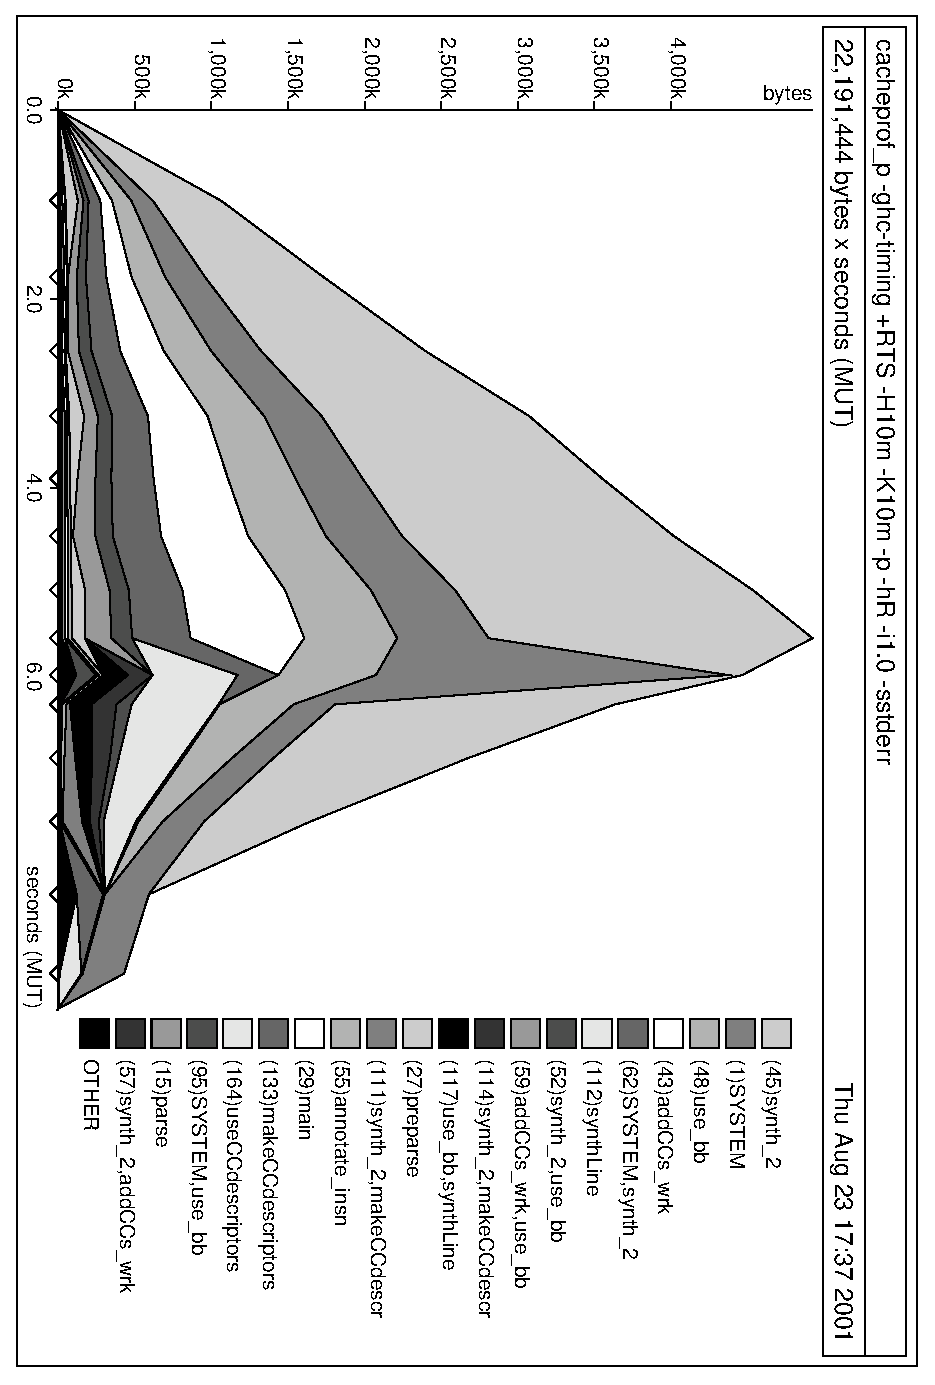
\epsfig{file=cacheprof_p.eps,width=5in}
\caption{A graph showing the progress of retainer profiling}
\label{fig-cacheprof}
\end{figure}

\section{Comparision with nhc}

\section{Files}

This section gives a summary of changes made to the GHC in 
implementing retainer profiling.
Only three files (@includes/StgRetainerProf.h@, @RetainerProfile.c@, and 
@RetainerProfile.h@) are new, and all others exist in the GHC.

@\includes@ directory:

\begin{description}
\item[StgRetainerProf.h] defines types @retainer@ and @retainerSet@. 
\item[Stg.h] includes the header file @StgRetainerProf.h@.
\item[Closures.h] changes structure @StgProfHeader@.
\item[Constants.h] changes constants @PROF_HDR_SIZE@, @SCC_UF_SIZE@, and
  @SCC_SEQ_FRAME_SIZE@.
\item[ClosureMacros.h] changes macros @SET_PROF_HDR()@ and 
  @SET_STATIC_PROF_HDR()@.
\item[Updates.h] changes macro @PUSH_STD_CCCS()@.
\end{description}

@\rts@ directory:

\begin{description}
\item[Exception.hc] changes constant @CATCH_FRAME_BITMAP@, 
\item[StgStartup.hc] changes constant @STOP_THREAD_BITMAP@.
\item[StgStdThunks.hc] changes constant @RET_BITMAP@.
\item[Updates.hc] changes constant @UPD_FRAME_BITMAP@.
\item[RetainerProfile.c] implements the retainer profiling engine.
\item[RetainerProfile.h] is the header for @RetainerProfile.c@.
\item[RetainerSet.c] implements the abstract datatype @retainerSet@.
\item[RetainerSet.h] defines the interface for @retainerSet@.
\item[GC.c] invokes @resetStaticObjectForRetainerProfiling()@ in 
  @GarbageCollect()@.
\item[Itimer.c] changes @handle_tick()@.
\item[ProfHeap.c] changes @initHeapProfiling()@ and @endHeapProfiling()@.
\item[Profiling.c] changes @initProfilingLogFile()@ and 
  @report_ccs_profiling()@.
\item[Proftimer.c] declares @ticks_to_retainer_profiling@, 
  @performRetainerProfiling@, and @doContextSwitch@.
\item[Proftimer.h] is the header for @Proftimer.c@. Defines @PROFILING_MIN_PERIOD@,
  which specifies the minimum profiling period and the default profiling period.
%\item[RtsAPI.c] implements @setRetainerField()@.
\item[RtsFlags.c] 
  sets @RtsFlags.ProfFlags.doHeapProfile@ and
  adds a string to  @usage_text[]@ in @setupRtsFlags()@.      
\item[RtsFlags.h] defines constants @HEAP_BY_RETAINER@ and @RETAINERchar@.
\item[RtsStartup.c] includes the header file @RetainerProfile.h@.
  Changes @shutdownHaskell()@.
\item[Schedule.c] changes @schedule()@. 
\item[Stats.c] 
  declares @RP_start_time@, @RP_tot_time@, @RPe_start_time@, 
  @RPe_tot_time@.
  Changes @mut_user_time_during_GC()@, @mut_user_time()@, 
  @stat_startExit()@, 
  @stat_endExit()@, and
  @stat_exit()@.
  Defines
  @mut_user_time_during_RP()@, 
  @stat_startRP()@, and
  @stat_endRP()@.
\item[Stats.h] is the header for @Stats.c@.
\item[StgMiscClosures.hc] redefines @stg_DEAD_WEAK_info@.
\item[Storage.c] changes @initStorage()@, @memInventory()@.
\end{description}

\bibliographystyle{plain}
\bibliography{reference}

\end{document}
